\documentclass{pclass}
\addbibresource{refs.bib}
\usepackage{url}

\typpracy{PRACA DYPLOMOWA MAGISTERSKA}
\author{Michał Olszewski}
\title{Tytuł pracy}
\tieng{Title}
\album{136009}
\studia{niestacjonarne}
\poziom{II}
\promotor{dr inż. Kamil Halbiniak}
%\epigrafquote{I’d rather write programs to write programs than write programs.}
%\epigrafsource{Richard Sites}
%\dedykacja{pracę dedykuje\\...}

\begin{document}

\frontpage
\setcounter{tocdepth}{1}

\cleardoublepage
\tableofcontents

\cleardoublepage
\chapter{Introduction}
\label{ch:introduction}

An initial compromise can enable further modeled reachability under a specified network topology and policy. In this thesis, the \emph{blast radius} is the set of resources reached by the simulator after an initial compromise; it is a model output, not a measurement of real attacker movement~\cite{ou05mulval}. Conventional vulnerability prioritization often uses the CVSS score published by FIRST.org~\cite{cvss31}. CVSS describes vulnerability severity characteristics; it does not establish real-world exploit likelihood.

This thesis investigates a context-graph and state-transition approach, informed by attack-graph literature: represent network topology and CVE data, simulate propagation by Monte Carlo sampling, and use simulated mission-impact and blast-radius outcomes to rank defensive actions. The system is implemented in \mintinline{elixir}|Elixir|, with a visualization front-end in \mintinline{elixir}|Phoenix.LiveView|. It compares equal-action-count defense strategies with conventional CVSS-priority ordering; no full-study empirical comparison is reported in this thesis.

\begin{quote}
	\itshape A vulnerability score characterizes a flaw. A context graph defines the actions permitted by a specified model.
\end{quote}

The remainder of this chapter frames the goal of the thesis and outlines its structure. Section~\ref{ch:intro:goal} states the goal and scope. Section~\ref{ch:intro:questions} lists the research questions. Section~\ref{ch:intro:structure} describes the organization of the remaining chapters, and points forward to the architecture diagram in Chapter~\ref{ch:design} and the evaluation protocol in Chapter~\ref{ch:evaluation}.

Chapter~\ref{ch:theory} defines the context graph, state-transition process, and modeled blast-radius quantity used throughout the thesis.

\section{Goal and scope of the thesis}
\label{ch:intro:goal}

The goal of the thesis is to design and implement a small system, and to specify a reproducible evaluation protocol for it. The primary outcome is the simulated mission impact of an attack; blast radius is a secondary safety outcome. The current scope is intentionally limited to a single-pass offline analysis of one fixed stylized topology, policy, and attacker model. Reachability is canonical segment policy with operational flows derived in memory, and segmentation removes a policy rule. Each supported defensive action has unit cost, so the budget counts actions rather than deployable cost. The evaluation compares equal-action-count defense strategies with CVSS-priority ordering within an approved three-tier topology-scale study; current code supports the fixed baseline and generic topology sources, but not frozen controlled variants. The scope cannot establish real lateral-movement behavior, cost-aware segmentation, sensitivity to topology density or attacker profiles, or general scalability beyond measured scenarios. Runtime NVD ingestion is deferred; the baseline scenario may combine a reviewed static NVD subset with synthetic catalog entries. Online re-evaluation under topology change, live-CVE feed integration, and multi-tenant operation are out of scope.

\section{Research questions}
\label{ch:intro:questions}

The work is organized around one main research question and two sub-questions, which determine the evaluation protocol:

\begin{enumerate}
	\item \textbf{Main.} Within controlled stylized network topologies, how do equal-action-count defense strategies differ from CVSS prioritization in reducing simulated mission impact?
	\item \textbf{Sub-question 1.} How does a pre-attack feasibility constraint change the selected defense plans and the directly measured operational loss?
	\item \textbf{Sub-question 2.} How does controlled growth in topology size affect the simulation, strategy-selection, and total-evaluation runtime, and the mission-impact ranking of equal-budget defense strategies?
\end{enumerate}

\section{Structure of the thesis}
\label{ch:intro:structure}

The thesis is organized into seven chapters. Chapter~\ref{ch:literature_review} surveys prior work on attack graphs and vulnerability prioritization. Chapter~\ref{ch:theory} establishes the theoretical background and serves as a visual-elements reference. Chapter~\ref{ch:design} presents the design. Chapter~\ref{ch:implementation} describes the implementation. Chapter~\ref{ch:evaluation} specifies the evaluation protocol. Chapter~\ref{ch:conclusion} summarizes the contributions and outlines future work.


\cleardoublepage
\chapter{Literature Review}
\label{ch:literature_review}

This chapter surveys prior work relevant to the thesis across five themes: attack-graph construction, probabilistic and Bayesian attack modeling, CVSS-based vulnerability prioritization, defense optimization and network hardening, and Monte Carlo methods for network security. The discussion identifies a research gap that the present work addresses: the absence of a system that combines stochastic attack-path simulation with automated defense optimization under a constrained budget and evaluates the result against conventional prioritization baselines.

\section{Attack-Graph Construction and Analysis}

The attack graph, as a formalism for reasoning about multi-step exploitation, was introduced by \citeauthor{phillips98}~\cite{phillips98}, who represented network configurations, vulnerabilities, and attacker capabilities in a directed graph and computed the set of reachable privilege states. This seminal work established the two core primitives that recur in all subsequent literature: nodes representing attacker or host states and edges representing possible exploitation steps.

\citeauthor{jha02two}~\cite{jha02two} formalized the distinction between two families of attack graphs that shape the design of every later tool. \emph{State-enumeration} graphs represent each node as a global system state (the set of all compromised hosts and obtained privileges), while \emph{assumption-based} graphs track only the logical dependencies between individual exploits. The former gives completeness at the cost of combinatorial explosion; the latter trades some precision for tractability.

\citeauthor{sheyner02}~\cite{sheyner02} automated attack-graph generation through symbolic model checking with NuSMV, constructing graphs from network topology, firewall rules, and vulnerability databases. Their tool produced complete state-enumeration graphs and introduced a security metric---the probability of an attacker reaching a given target---derived from edge weights. This work demonstrated that attack graphs could be built automatically, but the state-enumeration approach did not scale beyond a few hundred hosts.

\citeauthor{ou05mulval}~\cite{ou05mulval} addressed scalability with MulVAL, a logic-programming-based analyzer that uses Datalog inference to derive the set of reachable exploits from a set of facts describing the network. MulVAL belongs to the assumption-based family and generates graphs for networks of several thousand hosts in seconds. Its output is a dependency graph in which leaf nodes are configuration facts and intermediate nodes represent exploits or conditions.

\citeauthor{homer08netspa}~\cite{homer08netspa} developed NetSPA, which pre-computes a reachability map to avoid the exponential blow-up of state enumeration. NetSPA was designed for enterprise-scale networks of thousands of hosts and emphasizes a shortest-path variant that is fast but conservative---it underestimates the attacker's ability to traverse longer paths. The tool's practical focus on network reachability makes it the closest precursor to the graph-construction component of the present work.

Surveys by \citeauthor{lippmann05}~\cite{lippmann05} and \citeauthor{kaynar16}~\cite{kaynar16} catalogued more than fifty attack-graph construction methods and taxonomized them by representation, scalability, and analytical capability. Kaynar identified a recurring trade-off: tools that emphasize scalability tend to under-represent attacker capability, while tools that emphasize expressiveness sacrifice performance on real networks.

\section{Topological Vulnerability Analysis}

A separate line of work, beginning with \citeauthor{ammann02tva}~\cite{ammann02tva}, exploits the monotonicity assumption---that attackers never lose privileges---to make attack-graph construction polynomial in the number of exploits. Under this assumption, an attacker who exploits a vulnerability on host $A$ to reach host $B$ retains access to $A$, removing the need to track all combinations of compromised hosts. The resulting \emph{topological vulnerability analysis} (TVA) graph represents exploits as nodes and pre- and post-conditions as edges, producing a structure closer to a dependency graph than a state graph.

The multiple-prerequisite (MP) variant relaxes the strict monotonicity assumption in a controlled way by allowing exploits to require multiple preconditions before they can be attempted. \citeauthor{ingols06mpg}~\cite{ingols06mpg} provided an empirical comparison of MP graphs against state-enumeration and monotonic representations on laboratory networks of up to 250 hosts. They found that MP graphs capture most attack paths available to a realistic attacker while reducing construction time by an order of magnitude relative to full state enumeration.

\section{Probabilistic and Bayesian Attack Modeling}

The attack graphs discussed so far are deterministic: an edge either exists or does not. Real-world exploitation is probabilistic, depending on attacker skill, tool availability, and time budget. Several works address this by casting the attack graph as a probabilistic model.

\citeauthor{frigault08}~\cite{frigault08} combined Bayesian networks with topological attack graphs to produce a probabilistic security metric: the likelihood that a given target is compromised given evidence about initial footholds. Each exploit node in the attack graph becomes a random variable in the Bayesian network, with conditional probability tables derived from CVSS exploitability metrics. The resulting model supports both forward inference (predicting compromise spread) and backward inference (identifying the most likely entry points for a given observed compromise).

\citeauthor{poolsappasit12}~\cite{poolsappasit12} extended Bayesian attack graphs to dynamic security risk management. Their system recomputes compromise probabilities as vulnerabilities are patched or new exploits are discovered, allowing the defender to compare the marginal risk reduction of alternative defensive actions. This dynamic capability is the closest antecedent to the simulation-informed optimization loop in the present work, though their approach relies on analytic Bayesian inference rather than Monte Carlo sampling.

\section{CVSS-Based Vulnerability Prioritization}

The Common Vulnerability Scoring System~\cite{cvss31}, published by FIRST.org and used as the primary input to the U.S. National Vulnerability Database~\cite{nvd}, assigns each CVE a base score in $0$--$10$ derived from exploitability and impact metrics. CVSS is the industry standard for per-vulnerability prioritization and serves as one of the baselines against which the present work is compared.

CVSS-based prioritization has a known limitation that motivates this thesis: it scores vulnerabilities in isolation, with no representation of the network topology that determines whether a given vulnerability is reachable from a given entry point. \citeauthor{allodi14}~\cite{allodi14} demonstrated empirically that fixing vulnerabilities solely on the basis of high CVSS scores is statistically equivalent to random patching. Using a case-control study of 374 public exploits, they found that the existence of a published proof-of-concept exploit is a significantly better risk predictor than the CVSS score. This finding reinforces the argument that contextual information---network topology, reachability, and attacker positioning---must complement vulnerability scoring for effective prioritization.

\section{Defense Optimization and Network Hardening}

The problem of selecting a set of defensive actions to minimize attack impact under a cost constraint has been studied from several angles.

\citeauthor{noel03}~\cite{noel03} formulated network hardening as a minimum-cost set-covering problem on the exploit dependency graph. Given a set of initial conditions that must be disabled to prevent an attacker from reaching critical targets, their algorithm finds the cheapest combination of patches, firewall rule changes, and service deactivations that achieves this goal. The result is a single hardened configuration; the method does not produce a ranked list of incremental actions or account for probabilistic exploitation.

\citeauthor{wang06hardening}~\cite{wang06hardening} extended this line of work by introducing probabilistic weights on exploit edges and formulating the hardening problem as finding the minimum-cost set of removals that brings the cumulative probability of reaching a target below a specified threshold. Their approach accounts for the fact that exploit success is uncertain, but the optimization remains a single-shot computation: it solves for a target configuration, not for a budget-constrained sequence of actions evaluated by their marginal impact.

\citeauthor{albanese12}~\cite{albanese12} addressed the computational cost of hardening optimization by introducing a heuristic that prunes irrelevant portions of the attack graph before computing defenses. Their method reduces the search space by identifying ancestors of critical assets that do not lie on any feasible attack path, achieving orders-of-magnitude speedup on networks of several thousand hosts while maintaining solution quality close to the unpruned optimum.

The defense optimizer in this thesis differs from these works in two respects. First, it evaluates candidate actions through repeated Monte Carlo simulation rather than closed-form probability propagation, capturing attacker behavior that would be missed by analytic models. Second, it operates as a greedy, incremental loop that selects actions one at a time under a budget constraint, producing a ranked sequence rather than a single target configuration.

\section{Monte Carlo Methods for Network Security}

The blast-radius samples produced by the simulator in this work are bounded counts on a discrete graph and are not normally distributed. The Mann--Whitney $U$ test~\cite{mann47}, a non-parametric test for comparing two independent samples when the normality assumption does not hold, is therefore the appropriate choice for the comparative evaluation in Chapter~\ref{ch:evaluation}.

Monte Carlo simulation has been applied to network security in several contexts. \citeauthor{matthews21}~\cite{matthews21} developed stochastic simulation techniques for inference on Bayesian attack graphs, demonstrating that Monte Carlo methods scale more favorably than exact Bayesian inference for large graphs with dense dependency structures. Their approach is closely related to the simulation engine in the present work, though theirs focuses on inference within an existing Bayesian graph rather than on comparing defense strategies.

\section{Summary and Research Gap}

The surveyed literature demonstrates a consistent pattern: attack graphs make network-level reasoning about exploitation possible, but existing tools make a trade-off between analytic tractability and representational fidelity. Tools that use closed-form probability propagation (Bayesian attack graphs, minimum-cost hardening) can compute exact solutions, but their models simplify attacker behavior to conditional probability tables. Tools that use state enumeration or monotonicity can represent complex dependencies, but they do not integrate stochastic attacker simulation with incremental defense optimization.

This thesis addresses the gap by combining three elements not previously integrated: (1) a graph construction in the NetSPA/MP family that balances scalability with expressiveness, (2) a stochastic simulator that captures attacker behavior beyond what conditional probability tables can represent, and (3) a defense optimizer that evaluates candidate actions by their marginal impact on the simulated blast-radius distribution, producing a ranked sequence of recommendations under a constrained budget. The resulting system is evaluated against two baselines (CVSS-based and random prioritization) using the experimental methodology described in Chapter~\ref{ch:evaluation}.


\chapter{Theoretical Background}
\label{ch:theory}

This chapter is a \emph{visual-elements reference} for the rest of the thesis. Each section demonstrates one type of visual element supported by the document class, with a minimal but complete example that can be copied into another chapter. Where appropriate, the examples are drawn from the thesis topic --- attack-graph construction, blast-radius simulation, and defense optimization --- so that the chapter also serves as a worked example of the visual elements applied to a non-trivial domain.

\section{Attack Graphs and Their Visualization}

A figure is a floating environment that places a graphic at a suitable position on the page. The body of the figure is an \texttt{\textbackslash includegraphics} call (for a raster or vector image) or a TikZ picture. The image file must live in \texttt{img/} (or be referenced with a full path). The class \texttt{pclass.cls} also accepts an optional caption and label.

\begin{code}
	\begin{minted}{latex}
\begin{figure}[hbt!]
	\centering
	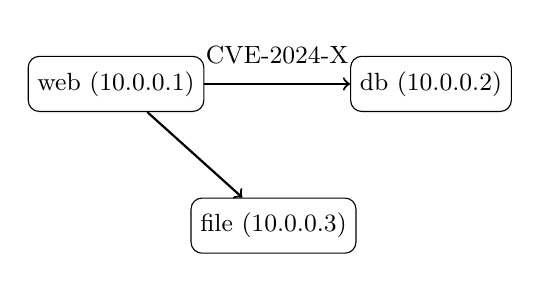
\begin{tikzpicture}[
		every node/.style={draw, rectangle, rounded corners, minimum width=2cm, minimum height=0.7cm, font=\small},
		arrow/.style={->, thick},
	]
	\node (h1) at (0, 1.2) {web (10.0.0.1)};
	\node (h2) at (4, 1.2) {db (10.0.0.2)};
	\node (h3) at (2, -0.6) {file (10.0.0.3)};
	\draw[arrow] (h1) -- node[above, draw=none, fill=none] {CVE-2024-X} (h2);
	\draw[arrow] (h1) -- (h3);
	\end{tikzpicture}
	\caption{Small attack graph: three hosts, two exploit edges.}
	\label{fig:attack-graph-example}
\end{figure}
	\end{minted}
	\caption{Source template for an attack-graph figure.}
	\label{src:theory:figure-template}
\end{code}

The example below uses the existing logo as a stand-in. In a real chapter, the image path would point at the actual result.

\begin{figure}[hbt!]
	\centering
	
\includegraphics[width=0.6\textwidth]{logo_wiisi.png}
	\caption{Placeholder figure: an attack-graph render produced by the system would replace this slot.}
	\label{fig:theory:figure-example}
\end{figure}

\section{Source Code Listings}

A source code listing is a floating environment based on \texttt{minted}. The class file \texttt{pclass.cls} defines a \texttt{code} environment that sets the listing type to \enquote{Source Code} and provides a caption and a label. The template (literal text, not active LaTeX) is:

\begin{quote}
	\texttt{\textbackslash begin\{code\}}\quad $\rightarrow$\quad \texttt{\textbackslash begin\{minted\}\{python\}}\quad $\rightarrow$\quad \emph{code body}\quad $\rightarrow$\quad \texttt{\textbackslash end\{minted\}}\quad $\rightarrow$\quad \texttt{\textbackslash caption\{...\}}\quad $\rightarrow$\quad \texttt{\textbackslash label\{src:...\}}\quad $\rightarrow$\quad \texttt{\textbackslash end\{code\}}
\end{quote}

\noindent A worked example in the Elixir language, showing a module that holds a single attack-graph node:

\begin{code}
	\begin{minted}{elixir}
defmodule NetworkDefense.AttackGraph.Node do
  @enforce_keys [:id, :host, :service, :vulnerabilities]
  defstruct id: nil, host: nil, service: nil, vulnerabilities: []

  def new(host, service, vulnerabilities) do
    %__MODULE__{
      id: "#{host}:#{service}",
      host: host,
      service: service,
      vulnerabilities: vulnerabilities
    }
  end

  def compromise_probability(%__MODULE__{vulnerabilities: vs}) do
    Enum.reduce(vs, 0.0, &max(&2, cvss_to_prob(&1.cvss)))
  end
end
	\end{minted}
	\caption{An attack-graph node module in Elixir.}
	\label{src:theory:elixir-example}
\end{code}

\noindent A worked example in the Python language, showing a min-cut finder on a tiny attack graph:

\begin{code}
	\begin{minted}{python}
def min_cut(graph, source, sink):
    """Stoer--Wagner min-cut, simplified for unweighted graphs."""
    remaining = set(graph.nodes)
    best_cut = float("inf")
    while len(remaining) > 1:
        weights = {n: 0 for n in remaining}
        in_tree = set()
        last, prev = None, None
        for _ in remaining:
            for n in remaining - in_tree:
                for (u, v) in graph.edges:
                    if u == n and v in in_tree:
                        weights[n] += 1
            chosen = max(remaining - in_tree, key=lambda n: weights[n])
            in_tree.add(chosen)
            prev, last = last, chosen
        cut = weights[last]
        if cut < best_cut:
            best_cut = cut
        graph = contract(graph, prev, last)
        remaining.remove(prev)
    return best_cut
	\end{minted}
	\caption{A min-cut implementation in Python.}
	\label{src:theory:python-example}
\end{code}

\section{Inline Code}

Inline code is typeset with \texttt{\textbackslash mintinline}. The first argument is the language, the second is the snippet:

\begin{itemize}
	\item \mintinline{elixir}|NetworkDefense.AttackGraph|
	\item \mintinline{elixir}|monte_carlo_step/3|
	\item \mintinline{python}|min_cut(graph, source, sink)|
\end{itemize}

\section{Tables}

The class loads \texttt{booktabs}, \texttt{multirow}, and \texttt{array}, so the standard patterns for academic tables are available. The simplest form is a three-column table with horizontal rules only:

\begin{table}[hbt!]
	\centering
	\begin{tabular}{lcr}
		\toprule
		\textbf{Strategy} & \textbf{Mean $|B|$} & \textbf{$p$-value} \\
		\midrule
		No defense     & 412 & ---      \\
		Random         & 388 & 0.21     \\
		CVSS-priority  & 274 & $< 0.01$ \\
		Proposed       & 153 & $< 0.01$ \\
		\bottomrule
	\end{tabular}
	\caption{Blast-radius comparison on a 200-host topology, $|V| = 200$.}
	\label{tab:theory:simple}
\end{table}

A wider table that combines \texttt{multirow} and \texttt{\textbackslash cline} is shown in Table~\ref{tab:theory:wide}. This is the pattern to use for benchmark results where a single row label spans multiple data rows.

\begin{table}[hbt!]
	\centering
	\begin{tabular}{lrrr}
		\toprule
		\textbf{Topology} & \textbf{Strategy} & \textbf{Mean $|B|$} & \textbf{Reduction ($\times$)} \\
		\midrule
		\multirow{2}{*}{Small (20 hosts)}  & No defense & 18  & 1.0  \\
		                                    & Proposed   & 5   & 3.6  \\
		\cline{2-4}
		\multirow{2}{*}{Large (1000 hosts)} & No defense & 980  & 1.0  \\
		                                    & Proposed   & 173  & 5.7  \\
		\bottomrule
	\end{tabular}
	\caption{Benchmark results on small and large topologies.}
	\label{tab:theory:wide}
\end{table}

\section{Diagrams with TikZ}

Diagrams are drawn with TikZ inside a \texttt{figure} environment. The example below is a small attack graph: each node is a host/service pair, and arrows show exploit opportunities. TikZ is sensitive to coordinate placement, so it is worth sketching the layout before committing to code.

\begin{figure}[hbt!]
	\centering
	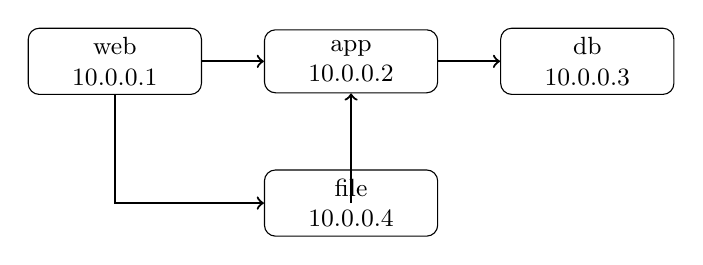
\begin{tikzpicture}[
			every node/.style={align=center, draw, rectangle, rounded corners, minimum width=2.2cm, minimum height=0.8cm, font=\small},
			arrow/.style={->, thick},
		]
		\node (a) at (0, 0)    {web\\10.0.0.1};
		\node (b) at (3.0, 0)  {app\\10.0.0.2};
		\node (c) at (6.0, 0)  {db\\10.0.0.3};
		\node (d) at (3.0, -1.8) {file\\10.0.0.4};

		\draw[arrow] (a) -- (b);
		\draw[arrow] (b) -- (c);
		\draw[arrow] (a) |- (d);
		\draw[arrow] (d) -| (b);
	\end{tikzpicture}
	\caption{Example TikZ diagram: a small attack graph.}
	\label{fig:theory:diagram}
\end{figure}

\section{Mathematics}

Inline math is delimited by \texttt{\$...\$} and display math by \texttt{\textbackslash[ ... \textbackslash]}. Equations can be numbered with the \texttt{equation} environment and aligned at a chosen relation with \texttt{align}.

Inline example: the probability that a single exploit of CVSS base score $s$ succeeds is $P = f(s)$, where $f$ is a monotone increasing function bounded above by $1$. The exact form of $f$ is an empirical question; one reasonable choice is $f(s) = s / 10$. Display example:

\[
P(\text{entry at } e \text{ reaches } v) \;=\; 1 - \prod_{(u, v) \in \text{path}} \bigl(1 - P(\text{exploit } (u, v))\bigr).
\]

Aligned example, useful for derivations:

\begin{align*}
	\mathrm{E}[B \mid e]  &= \sum_{h \in V} P(\text{reach } h \mid e) \\
	                      &= \sum_{h \in V} \Bigl( 1 - \prod_{(u, v) \in \pi_e(h)} \bigl(1 - f(s_{uv})\bigr) \Bigr).
\end{align*}

\section{Lists}

The class loads \texttt{enumitem}, which makes it easy to adjust list spacing. A simple itemized list:

\begin{itemize}
	\item Attack-graph construction.
	\item Monte Carlo blast-radius simulation.
	\begin{itemize}
		\item Stochastic propagation.
		\item Per-host compromise sampling.
	\end{itemize}
	\item Defense optimization.
\end{itemize}

A simple enumerated list:

\begin{enumerate}
	\item Ingest network topology.
	\item Enrich nodes with CVE / CVSS data.
	\item Build the attack graph.
	\item Run Monte Carlo simulation.
	\item Compute blast-radius map.
	\item Run optimizer (min-cut, greedy, or hybrid).
\end{enumerate}

A list with \texttt{\textbackslash enquote} strings around phrases:

\begin{itemize}
	\item The simulator is described as \enquote{stochastic, monotonic, and conservative}.
	\item The user provides \enquote{only the network topology and a CVE feed}.
\end{itemize}

\section{Quotes and Epigraphs}

A short quotation is set with the \texttt{quote} environment. The block is indented on both sides and the text is set in \enquote{quotation marks}:

\begin{quote}
	\itshape The best way to find out if a network is secure is to assume it isn't, and to ask what an attacker would do.
\end{quote}

The class also provides a local \texttt{\textbackslash epigraph} command that can be used inside a chapter to set an attributed quotation apart from the body text. The class file declares an \texttt{\textbackslash epigraph} macro from the \texttt{epigraph} package.

\begin{code}
	\begin{minted}{latex}
\epigraph{To be or not to be, that is the question.}{Shakespeare}
	\end{minted}
	\caption{Template for an in-chapter epigraph.}
	\label{src:theory:epigraph-template}
\end{code}

The rendered form is:

\epigraph{To be or not to be, that is the question.}{Shakespeare}

\section{Footnotes}

A simple footnote uses \texttt{\textbackslash footnote} and runs in the same paragraph as the reference. A footnote that is referenced from a position that is awkward for a marginal note (for example, after a list) can be deferred to the bottom of the page with \texttt{\textbackslash footnotetext} and a matching \texttt{\textbackslash footnote} placeholder.

A single-line footnote example: this is a sentence with a footnote\footnote{This is the footnote text; it appears at the bottom of the page.} attached.

A multi-line footnote using \texttt{\textbackslash footnotetext}:

\footnotetext{This is a longer footnote. It can span multiple lines, contain its own paragraph breaks, and even contain inline code such as \mintinline{elixir}|NetworkDefense.Optimizer.min_cut/2|, as long as the surrounding text is not overly fragile.}


\chapter{Design and Methodology}
\label{ch:design}

This chapter presents the design of the system. The goals collected in Section~\ref{ch:design:goals} drive the structure, which is then described in three layers: data, simulation, and optimization. The relationship between the layers is captured in Figure~\ref{fig:design:architecture}, and the requirements are summarized in Table~\ref{tab:design:requirements}.

\begin{figure}[hbt!]
	\centering
	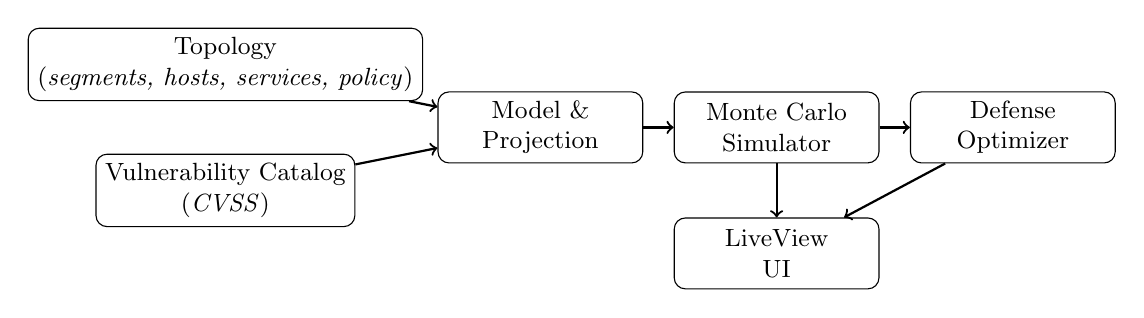
\begin{tikzpicture}[
			every node/.style={align=center, draw, rectangle, rounded corners, minimum width=2.6cm, minimum height=0.9cm, font=\small},
			arrow/.style={->, thick},
		]
		\node (topo)   at (0,  0)   {Topology\\(\textit{segments, hosts, services, policy})};
		\node (cve)    at (0,  -1.6) {Vulnerability Catalog\\(\textit{CVSS})};
		\node (graph)  at (4.0, -0.8) {Model \&\\Projection};
		\node (sim)    at (7.0, -0.8) {Monte Carlo\\Simulator};
		\node (opt)    at (10.0, -0.8) {Defense\\Optimizer};
		\node (ui)     at (7.0, -2.4) {LiveView\\UI};

		\draw[arrow] (topo)  -- (graph);
		\draw[arrow] (cve)   -- (graph);
		\draw[arrow] (graph) -- (sim);
		\draw[arrow] (sim)   -- (opt);
		\draw[arrow] (sim)   -- (ui);
		\draw[arrow] (opt)   -- (ui);
	\end{tikzpicture}
	\caption{Pipeline architecture: from data sources to optimizer and UI.}
	\label{fig:design:architecture}
\end{figure}

\section{Design Goals}
\label{ch:design:goals}

The system is designed to satisfy a small set of explicit goals. The goals are partitioned into functional and non-functional groups.

\begin{itemize}
	\item \textbf{Functional:}
	\begin{itemize}
		\item Construct a canonical graph with segment-policy reachability and derive operational flows for simulation.
		\item Simulate attacker propagation by Monte Carlo sampling and produce blast-radius and mission-impact outcomes.
		\item Recommend defensive actions (segment-policy removals, vulnerability patches) intended to reduce the modeled mission impact, with blast radius as a secondary safety outcome.
	\end{itemize}
	\item \textbf{Non-functional:}
	\begin{itemize}
		\item Reproducible results: a given topology and seed must produce the same blast-radius map across runs.
		\item Measurable scale: a benchmark over three controlled topology-size tiers must report median simulation, strategy-selection, and total-evaluation durations on a fixed documented environment after warm-up; no general scalability claim is made without such measurements.
		\item Implementation fits in a small number of Elixir source files, to make the system easy to study and modify~\cite{ou05mulval}.
	\end{itemize}
\end{itemize}

A compact view of the design is given in Table~\ref{tab:design:requirements}, which lists each requirement together with the section that elaborates on it.

\begin{table}[hbt!]
	\centering
	\begin{tabular}{lll}
		\toprule
		\textbf{ID} & \textbf{Requirement}            & \textbf{Elaboration} \\
		\midrule
		R1 & Topology ingest                 & Section~\ref{ch:design:data}       \\
		R2 & Vulnerability catalog           & Section~\ref{ch:design:data}       \\
		R3 & Context-graph construction      & Section~\ref{ch:design:graph}      \\
		R4 & Monte Carlo simulation          & Section~\ref{ch:design:sim}        \\
		R5 & Policy-based segmentation        & Section~\ref{ch:design:opt}        \\
		R6 & Greedy patch prioritization     & Section~\ref{ch:design:opt}        \\
		R7 & Annealing optimization            & Section~\ref{ch:design:opt}        \\
		R8 & LiveView-based UI               & Section~\ref{ch:design:ui}         \\
		\bottomrule
	\end{tabular}
	\caption{Design requirements and where each is elaborated in this chapter.}
	\label{tab:design:requirements}
\end{table}

\section{Data Layer}
\label{ch:design:data}

The data layer consists of two inputs. The first is a \emph{network topology}: a set of network segments, hosts, and services, together with a segment-to-segment reachability policy. Each policy rule permits the source segment to initiate traffic to matching services in the target segment and carries protocol and port-range data. The second is a \emph{vulnerability catalog} containing CVSS data and a separately assigned success probability. Generated topologies use a synthetic catalog. The fixed baseline may use a reviewed static NVD subset; a live NVD feed is not part of the implementation. CVSS describes severity characteristics, not a calibrated probability or real-world exploit likelihood~\cite{nvd}.

\section{Context-Graph Layer}
\label{ch:design:graph}

The graph layer stores the topology as a typed context graph. Hosts, services, and network segments are nodes; ownership (segment contains host, host runs service) and reachability are edges. Reachability is segment policy, not a host/service flow: the stored edge connects a source to a target segment and carries protocol and port-range data. The effective \enquote{host to service} flow is a deterministic projection materialized in memory when the simulator or the network view needs it. No flow is admitted unless a policy rule supports it, and no complete static attack graph is enumerated before simulation. The context graph and state-transition simulation are informed by attack-graph literature, including MulVAL~\cite{ou05mulval} and multiple-prerequisite graphs~\cite{ingols06mpg}; they are not an implementation of either attack-graph family.

\section{Simulation Layer}
\label{ch:design:sim}

The simulation layer runs a fixed number of Monte Carlo trials. Each trial starts at the configured entry point. At each state transition, the simulator evaluates eligible actions, selects one uniformly, then samples its outcome. Exploit actions use the vulnerability's independently assigned, stylized success probability; credential actions are deterministic when their preconditions hold. The probability is not derived from CVSS and is not calibrated to real-world exploitation. One trial reports its final set of compromised host footholds, including the initial foothold. The aggregate report gives their count distribution and the per-host empirical compromise probability.

\section{Optimization Layer}
\label{ch:design:opt}

The optimization layer takes simulated mission-impact and blast-radius outcomes with a budget $k$ of defensive actions. It returns actions selected under the configured objective. The thesis uses mission impact as the primary outcome and blast radius as a secondary safety outcome. Every current action has unit cost, so $k$ is an equal-action-count budget rather than a deployment-cost model. Simulation-informed and annealing strategies score candidates through simulation; CVSS-priority and topology-based strategies use direct rankings:

\begin{itemize}
	\item \textbf{Policy segmentation.} Remove a segment-policy rule. Each removal is a single canonical policy change, not a cut of individual host edges; the topology-based strategy ranks it by the reduction in deterministically reachable hosts after re-materializing the flows.
	\item \textbf{Simulation-informed patching.} Rank vulnerabilities by their marginal reduction under the selected simulation objective, measured by re-simulating each candidate graph, and patch the highest-ranked ones up to the budget.
	\item \textbf{Simulated annealing.} A stochastic search over patching and segmentation actions, guided by the selected simulated objective for each candidate graph.
\end{itemize}

\section{UI Layer}
\label{ch:design:ui}

The UI layer is a Phoenix LiveView application. It lets the user edit a graph, run simulations and optimizations, and inspect their reports. A simulation report can show a blast-radius heat map with mission-impact results.


\chapter{Implementation}
\label{ch:implementation}

This chapter describes the implementation of the system. The description follows the layering established in Chapter~\ref{ch:design}: the data layer, the attack-graph layer, the simulation layer, the optimization layer, and the UI layer. The implementation is small enough to be discussed end-to-end, and the most important parts are illustrated with code excerpts.

\section{Attack-Graph Layer}

The attack-graph layer is implemented as a small set of Elixir modules. The central data structure is a directed graph whose nodes are \mintinline{elixir}|%NetworkDefense.AttackGraph.Node{}| records and whose edges are \mintinline{elixir}|%NetworkDefense.AttackGraph.Edge{}| records. The graph is built in two passes: a structural pass that follows the network reachability relation, and an enrichment pass that adds edges for each applicable CVE. Source Code~\ref{src:impl:graph} shows the entry point of the graph builder.

\begin{code}
	\begin{minted}{elixir}
defmodule NetworkDefense.AttackGraph do
  alias NetworkDefense.AttackGraph.{Node, Edge}

  def build(topology, cve_feed) do
    base_nodes = topology.hosts
                 |> Enum.flat_map(&host_service_nodes/1)
    base_edges = topology.reachability
                 |> Enum.flat_map(&reachability_edges/1)
    enriched_edges = base_edges
                     |> Enum.flat_map(&cve_edges(&1, cve_feed))
    %{nodes: base_nodes, edges: base_edges ++ enriched_edges}
  end
end
	\end{minted}
	\caption{Entry point of the attack-graph builder.}
	\label{src:impl:graph}
\end{code}

The choice of a two-pass construction is deliberate: it keeps the structural and enrichment concerns in separate functions, and it makes it easy to add a third pass later (e.g., for transitive-vulnerability inference) without changing the upstream passes.

\section{Simulation Layer}

The simulation layer is implemented as a single \mintinline{elixir}|NetworkDefense.Simulator| module. The module exposes a \mintinline{elixir}|run/3| function that takes a graph, an entry point, and a number of iterations, and returns a blast-radius map. The pipeline is illustrated in Figure~\ref{fig:impl:pipeline}.

\begin{figure}[hbt!]
	\centering
	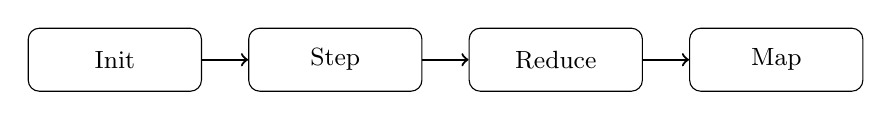
\begin{tikzpicture}[
			every node/.style={align=center, draw, rectangle, rounded corners, minimum width=2.2cm, minimum height=0.8cm, font=\small},
			arrow/.style={->, thick},
		]
		\node (p1) at (0, 0) {Init};
		\node (p2) at (2.8, 0) {Step};
		\node (p3) at (5.6, 0) {Reduce};
		\node (p4) at (8.4, 0) {Map};

		\draw[arrow] (p1) -- (p2);
		\draw[arrow] (p2) -- (p3);
		\draw[arrow] (p3) -- (p4);
	\end{tikzpicture}
	\caption{The four stages of the simulator pipeline.}
	\label{fig:impl:pipeline}
\end{figure}

The simulator step itself is shown in Source Code~\ref{src:impl:step}. It is a small recursive function over the attack graph; the recursion is bounded by the iteration budget and the depth of the graph.

\begin{code}
	\begin{minted}{elixir}
defp step(graph, current, reached, depth) do
  outgoing = outgoing_edges(graph, current)

  case Enum.random(outgoing) do
    nil ->
      reached

    edge ->
      if :rand.uniform() < edge.probability and depth > 0 do
        step(graph, edge.target, MapSet.put(reached, edge.target), depth - 1)
      else
        reached
      end
  end
end
	\end{minted}
	\caption{One step of the Monte Carlo simulator.}
	\label{src:impl:step}
\end{code}

\section{Optimization Layer}

The optimization layer is implemented in three sibling modules, one per strategy:

\begin{itemize}
	\item \mintinline{elixir}|NetworkDefense.Optimizer.MinCut|
	\item \mintinline{elixir}|NetworkDefense.Optimizer.Greedy|
	\item \mintinline{elixir}|NetworkDefense.Optimizer.Hybrid|
\end{itemize}

\noindent Each module exposes a \mintinline{elixir}|recommend/2| function with the same signature, so they are interchangeable at the call site.

The min-cut strategy is implemented in terms of a small Stoer--Wagner implementation; the greedy strategy is implemented in terms of a sort over the marginal blast-radius reduction of each vulnerability. The hybrid strategy alternates the two and uses the better of the two at each step.

A small auxiliary routine, \mintinline{elixir}|marginal_reduction(graph, blast_map, action)|, encapsulates the cost of evaluating a single candidate action. Listing it here is not necessary for the narrative; what matters is that the call site in the optimizer loop is a single line.

\section{UI Layer}

The UI layer is a Phoenix LiveView application. The main page renders the current blast-radius map as a heat map, lists the top recommended defensive actions, and shows a side-by-side comparison of the current and post-defense blast-radius maps. The user can step through the recommended actions one at a time, and the visualization updates in real time as each action is applied.

The choice of LiveView is driven by the need for low-latency interaction: the user typically wants to see the effect of each candidate action immediately, and a full HTTP round-trip per action would be too slow.


\chapter{Evaluation}
\label{ch:evaluation}

This chapter specifies the evaluation protocol for the system. No full-study empirical result is reported in this thesis. The protocol defines the evidence required before comparing strategies.

\section{Methodology}

The current evaluation scope is a fixed stylized topology, segment-policy configuration, and attacker model. It cannot support claims about real lateral movement, topology- or vulnerability-density sensitivity, attacker-profile sensitivity, or general scalability. All current defensive actions have unit cost, so the budget compares equal action counts; it does not represent deployable, cost-aware segmentation. The current code supports the fixed baseline scenario and generic topology sources; the controlled topology-size tiers of the approved scale study are a research design and are not yet implemented as frozen study inputs.

A reproducible evaluation must provide a versioned runner; the exact topology, policy, vulnerability catalog, mission capabilities and required flows, entry point, and simulation configuration; the seed schedule; the selected action list, including random choices, and budget; complete per-trial outcomes; and the aggregation and statistical-analysis code. Each strategy must be run against the same declared scenario and equal action-count budget. The compared strategies are random selection, CVSS-priority ordering, topology-driven policy segmentation, simulation-informed patching, and simulated-annealing search over both action classes, each under equal action-count budgets of one through three with multiple fixed selection seeds.

The primary measure is the simulated mission impact across trials; blast radius is a secondary safety outcome computed from the same trials. Feasibility is compared on paired constrained and unconstrained plans, reporting pre-attack feasibility, unavailable required flows, and affected mission capabilities. Paired scenario and evaluation seeds are used so that compared plans differ only in the applied constraint. Runtime, memory use, and convergence may be reported only on a fixed documented environment after warm-up. If independently sampled groups are compared, the Mann--Whitney $U$ test~\cite{mann47} may be appropriate. Matched seeds or paired scenarios require a paired analysis selected before examining results.

\section{Results}

Results are pending the artifacts specified above. No percentage reduction, statistical conclusion, calibration claim, or comparison between strategies is supported until those artifacts are available.

\section{Strategy Comparison}

The protocol compares the available strategies on the declared fixed scenario, using the same entry point, seed schedule, and equal action-count budget. A comparison must report the full action list as well as mission-impact outcomes. It must not interpret lower modeled mission impact as evidence of real-world defensive effectiveness.

\section{Discussion}

The system is a context graph plus state-transition simulation informed by attack-graph literature, not a NetSPA or multiple-prerequisite attack-graph implementation. CVSS data describes severity characteristics. The simulator instead uses independently assigned, stylized success probabilities and uniformly selects eligible actions; it is neither calibrated to, nor a predictor of, real-world exploit likelihood.

The fixed stylized topology, policy, attacker model, mission capabilities, and unit action costs are deliberate model boundaries. They preclude conclusions about real attack propagation, cost-aware deployable segmentation, density or profile sensitivity, and scalability beyond explicitly measured scenarios. The contribution is a controlled simulation comparison of ranking strategies under a feasibility constraint; it is not a claim that multi-objective hardening or mission-impact assessment is new.


\chapter{Conclusion}
\label{ch:conclusion}

The thesis set out to investigate a graph-based attack-simulation pipeline and automated defense optimizer. The implementation described in Chapter~\ref{ch:implementation} provides a context-graph model, state-transition simulation, and defense strategies. Chapter~\ref{ch:evaluation} defines the evidence required to assess them; it does not report empirical findings.

\section{Summary}
\label{ch:conclusion:summary}

Three contributions were made. First, a \emph{context graph} and state-transition model informed by attack-graph literature, with synthetic CVSS data and independently assigned success probabilities. Second, a \emph{Monte Carlo blast-radius simulator} for the fixed stylized attacker model. Third, a small \emph{optimization framework} supporting policy-rule segmentation, simulation-informed patching, and annealing-based search. Table~\ref{tab:conclusion:contributions} summarizes the contributions and their status.

\begin{table}[hbt!]
	\centering
	\begin{tabular}{lll}
		\toprule
		\textbf{Area}             & \textbf{Contribution}                          & \textbf{Status}      \\
		\midrule
		Context graph             & Informed by attack-graph literature            & Implemented          \\
		Monte Carlo simulation    & Uniform action selection, stylized outcomes    & Implemented          \\
		Optimization framework    & Unit-cost patching, segmentation, and annealing & Implemented         \\
		Empirical evaluation      & Reproducible protocol and reporting requirements & Pending             \\
		\bottomrule
	\end{tabular}
	\caption{Contributions of the thesis and their status.}
	\label{tab:conclusion:contributions}
\end{table}

\section{Future Work}
\label{ch:conclusion:future}

Several directions are left open for future work:

\begin{itemize}
	\item \textbf{Real-CVE integration.} The current vulnerability catalog is synthetic. A live NVD integration~\cite{nvd} would require a separate, justified mapping from CVE data to model parameters; CVSS must not be treated as a calibrated exploit probability.
	\item \textbf{Dynamic topology.} The present system assumes a static network. Extending the attack-graph and simulator layers to handle changes in the network over time would unlock operational use cases (e.g., daily re-evaluation of a corporate network).
	\item \textbf{Richer attacker models.} The current Monte Carlo simulator has one stylized model and no attacker-profile parameter. A more expressive model, perhaps informed by incident data, would require separate validation before it could support claims about attacker behavior~\cite{jha02two, ammann02tva}.
	\item \textbf{Better diagnostics.} Translating the optimizer's recommendations back to source-level positions in the input topology (e.g., \enquote{segment the link between $H_3$ and $H_7$, patch CVE-2024-1234 on $H_{12}$}) would substantially improve the usability of the system for security operators.
\end{itemize}

\section{Personal Growth}
\label{ch:conclusion:growth}

Beyond the technical contributions, the project was a useful exercise in keeping a small, focused design coherent as the surface area grew. The act of writing examples that double as documentation forced several early design decisions to be revisited; in every case the result was a cleaner interface.

\begin{quote}
	\itshape A security tool is only as good as the assumptions it makes explicit. The blast-radius number on its own is not a defense; the act of computing it forces the defender to make the assumptions visible.
\end{quote}


\cleardoublepage

\printbibliography
\addcontentsline{toc}{chapter}{\bibname}

\listoffigures
\addcontentsline{toc}{chapter}{\listfigurename}

\listoftables
\addcontentsline{toc}{chapter}{\listtablename}

\listoflistings
\addcontentsline{toc}{chapter}{\listoflistingsname}

\chapter*{Streszczenie}
\addcontentsline{toc}{chapter}{Streszczenie}

Streszczenie pracy.

\chapter*{Abstract}
\addcontentsline{toc}{chapter}{Abstract}

Thesis abstract.

\chapter*{Keywords}
\addcontentsline{toc}{chapter}{Keywords}

metaprogramming, smalltalk, language grammar, computer graphics, parallel, gpu programming, high performance computing, hpc


\oswiadczenie

\end{document}
